\section{Model View Controller}


Das Model View Controller Pattern teilt eine interaktive Anwendung in drei Komponenten. Das Model enthält die Grundfunktionalität und Daten. Views zeigen die Informationen dem Benutzer an. Controllers verarbeiten die Benutzereingaben. Views und Controller bilden zusammen die Benutzerschnittstelle. Durch einen Change-Propagation Mechanismus wird die Konsistenz zwischen der Benutzerschnittstelle und dem Model sichergestellt.

\subsection*{Example}


Software welche Daten von politischen Wahlen proportional mit verschiedenen Diagrammen darstellt.

UInt1 Miniprojekt

\subsection*{Context}


Interaktive Anwendungen mit einer flexiblen Benutzerschnittstelle.

\subsection*{Problem}


Benutzerschnittstellen sind anfällig für Änderungsanforderungen. Verschiedene Benutzer haben konkurierende Anforderungen an die Benutzerschnittstelle. Ein System mit der notwendigen Flexiblität ist teuer und fehleranfällig, falls die Benutzerschnittelle eng mit dem funktionellen Kern verwoben ist. Dies resultiert in der Notwendigkeit mehrere substentiell verschiedene Softwaresysteme zu entwickeln und zu unterhalten, eines für jede Benutzerschnittstellen-Implementierung. Folglich breiten sich Änderungen über viele Module aus.

\subsection*{Forces}


\begin{itemize}
	\item Die gleiche Information wird unterschiedlich in verschiedenen Fenstern angezeigt.
	\item Die Anzeige und das Verhalten der Anwendung muss Änderungen an den Daten unverzüglich widerspiegeln.
	\item Änderungen an der Benutzerschnittstelle sollen einfach sein, und auch möglich während der Laufzeit.
	\item Unterstützung für verschiedene "Look and Feel" Standards oder das Portieren der Benutzerschnittstelle soll nicht den Code im Kern der Applikation beeinflussen.
\end{itemize}

\subsection*{Solution}


Model-View-Controller (MVC) unterteilt eine Interaktive Anwendung in drei Bereiche: Verarbeitung, Ausgabe und Eingabe.

Die Model-Komponente kapselt die Kern-Daten und -Funktionalität. Das Modell ist unabhängig von spezifischen Ausgaberepräsentationen oder Eingabeverhalten.

Die View-Komponenten zeigen Informationen dem Benutzer an. Eine View erhält die Daten vom Model. Es sind mehrere Views des Models möglich.

Jede View hat eine zugehörige Controller Komponente. Controller verarbeiten Eingaben, normalerweise als Events. Events werden in Service-Requests übersetzt für das Model oder die View. Der Benutzer interagiert mit dem System nur über Controller.

Die Separation des Models von den View- und Controller-Komponenten erlaubt  verschiedene Darstellungen des selben Models. Wenn ein Benutzer das Model über einen Controller einer View verändert, müssen andere Views welche von diesen Daten abhängig sind, die Änderung wiedergeben. Dieser Propagation-Mechanismus ist im Publisher-Subscriber Pattern beschrieben.

\subsection*{Structure}


Die Model-Komponente enthält den funktionalen Kern der Anwendung. Der Change-Propagation Mechanismus verwaltet ein Register der abhängigen Komponente im Model. Alle Views und ausgewählte Controller registrieren ihr Bedürfnis über Änderungen informiert zu werden. Änderungen am Zustand des Models lösen den Change-Propagation Mechanismus aus. Dieser ist die einzige Verbindung zwischen dem Model und den Views und den Controllers.

View Komponenten präsentieren Informationen dem Benutzer. Verschiedene Views präsentieren die Information des Models auf unterschiedliche Arten. Jede View definiert eine Update Prozedur welche aktiviert wird vom Change-Propagation Mechanismus. Wird diese aufgerufen erhält die View die aktuellen Datenwerte vom Model und zeigt diese an.

Während der Initialisierung werden alle Views mit dem Model verbunden und beim Change-Propagation Mechanismus registriert. Zwischen Views und Controllers existiert eine eins-zu-eins Beziehung. Views besitzen oft Funktionalität welches es den Controllers erlaubt die Anzeige zu verändern. Dies ist nützlich für anwendergesteuerte Operationen welche das Model nicht verändern, wie zum Beispiel das Scrollen.

Die Controller Komponenten akzeptieren Benutzereingaben als Ereignisse (Events). Ereignisse werden in Anfragen an das Model oder den verbunden Controller übersetzt.

Falls das Verhalten eines Controllers abhängig ist vom Zustand des Models, dann registriert sich der Controller selbst beim Change-Propagation Mechanismus und implementiert eine Update-Prozedur.

\begin{figure}[H]
	\centering
	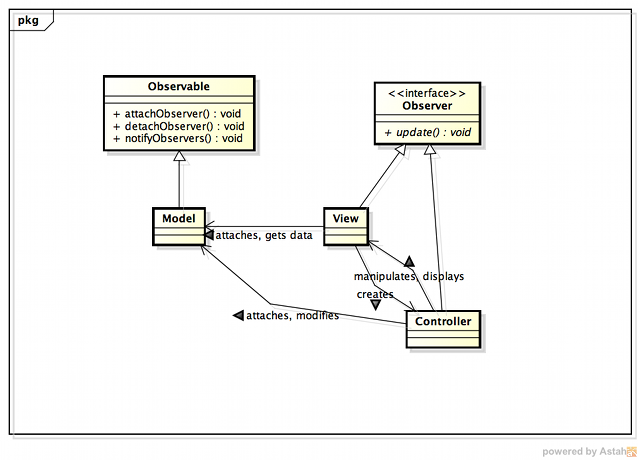
\includegraphics[width=0.7\textwidth]{content/posa1/images/mvc-classes.png}
	\caption{MVC Klassendiagramm}
\end{figure}


\subsection*{Dynamics}


\subsubsection*{Change Propagation}


:: UML von Seite 130 ::

\begin{itemize}
	\item Der Controller akzeptiert Benutzereingaben und aktiviert eine Service Prozedur des Models.
	\item Das Model führ den angeforderten Service aus. Dadurch werden interne Daten geändert.
	\item Das Model benachrichtigt alle registrierten Views und Controllers über den Change-Propagation Mechanismus.
	\item Jede View fordert die geänderten Daten vom Model an und Zeigt sie selbst auf dem Bildschirm an.
	\item Jede registrierte View empfängt Daten vom Model um gewisse Benutzerfunktionen ein- oder auszuschalten.
	\item Der ursprüngliche Controller erhält die Kontrolle wieder zurück.
\end{itemize}

\subsubsection*{Initialization}


:: UML von Seite 131 ::

\begin{itemize}
	\item Die Model-Instanz wird erzeugt, welche selbst interne Datenstrukturen initialisiert.
	\item Ein View-Objekt wird erzeugt. Diese erhält eine Referenz auf das Model als Parameter für die Initialisierung.
	\item Die View registriert sich beim Change-Propagation Mechanismus des Models.
	\item Die View fährt weiter mit der Initialisierung und erstellt seinen Controller. Sie übergibt Referenzen von sich selbst und dem Model an die Initialisierungs-Prozedur des Controllers.
	\item Der Controller registriert sich ebenfalls beim Change-Propagation Mechanismus des Models.
	\item Nach der Initialisierung fängt die Anwendung an Ereignisse zu verarbeiten.
\end{itemize}


\subsection*{Implementierung}


\begin{enumerate}
	\item  Trenne Benutzerinteraktion von der Kern-Funktionalität.
	\item  Implementiere den Change-Propagation Mechanismus. -> Publish-Subscribe Pattern
	\item  Entwirf und implementiere die Views.
	\item  Entwirf und implementiere die Controllers
	\item  Entwirf und implementiere die Beziehung zwischen View und Controller.
	\item  Implementiere den Aufbau von MVC.
	\item  Dynamische View erzeugung. Falls die Anwendung dynamisches öffnen und schliessen von Views erlaubt ist es eine gute Idee eine Komponente für die Verwaltung der Views bereitzustellen. -> View Handler Design Pattern
	\item  'Pluggable' Controllers. Die Trennung der Kontrollaspekte von der view erlaubt es verschiedene Controller mit einer View zu kombinieren. (zB Controller welcher Eingaben ignoriert -> Read Only View)
	\item  Infrastruktur für hierarchische Views und Controllers. Ein Framework welches auf MVC basiert implementiert wiederverwendbare View und Controller Klassen. Dies wir meist für häufig verwendete Benutzerschnittstellen-Elemente gemacht, wie Schaltflächen, Menüs oder Texteditoren. Die Benutzerschnittstelle wird dann grösstenteils aus der Kombinieren von vorgefertigten View-Objekten konstruiert.
	\item Weitere Entkopplung von Systemabhängigkeiten. Ein Framework mit einer sorgfältig erarbeiteten Sammlung von View und Controller-Klassen ist aufwändig zu erstellen. Deshalb will man diese Klassen möglichst Plattform-unabhängig machen. Man kann eine weitere Stufe von Indirektion (another level of indirection) zwischen dem System und der darunterliegenden Plattform durch das Anwenden des Bridge Patterns zur Verfügung stellen.
\end{enumerate}


Document-View: Weniger Trennung von Controller und View, da diese oft sowieso sehr ineinander verwoben sind.

\subsection*{Known Uses}


\begin{itemize}
	\item Smalltalk
	\item MFC
	\item ET++
	\item Zahlreiche Web Frameworks (ASP.NET MVC, Symfony, Ruby on Rails, Spring...)
	\item Frontend JavaScript Frameworks (AngularJS, Backbone...)
\end{itemize}

\subsection*{Consequences}


\subsubsection*{Benefits}


\begin{itemize}
	\item Unterschiedliche Sichten auf das selbe Model
	\item Views sind synchronisiert (Änderungen in Fenster A werden im Fenster B in Echtzeit aktualisiert)
	\item View und Controller eines Models können einfach ausgewechselt werden (u.U. sogar zur Laufzeit)
	\item "Look and Feel" kann angepasst werden -> Portierungen auf anderes Betriebssystem sind relativ einfach möglich
	\item Eignet sich als Grundlage für Application Frameworks (wie bei sehr vielen Web Frameworks bestätigt wurde)
\end{itemize}

\subsubsection*{Liabilities}


\begin{itemize}
	\item Erhöhte Komplexität; Controller und Views für einfach Menüs blasen das System auf ohne einen grossen Nutzen zu bringen
	\item Sehr viele Updates möglich; einfache Benutzeraktionen können zu sehr vielen Notifies führen. Deshalb sollten unnötige Notifications unterdrückt und Observer abgemeldet werden
	\item Enge Beziehung zwischen View und Controller; obwohl View und Controller separate Komponenten sind, ist ihre Verwendung ohne das entsprechende Gegenstück unwahrscheinlich
	\item Hohe Kopplung zwischen View/Controller und dem Model; Änderungen im Model wirken sich fast zwangsläufig auf alle Views und Controller aus.
	\item Ineffizienter Datenzugriff von Views; je nachdem wie der Datenzugriff geregelt ist (z.B. über getter pro Property) müssen pro Update eines Views sehr viele Methoden aufgerufen werden
	\item Abhängigkeiten zur Benutzerschnittstelle der Plattform sind in View und Controller abgebildet -> Protierung kann Änderungen in allen Views und Controller nach sich ziehen. Dies kann durch eine Abstraktion der Betriebssystemabhängigkeiten verhindert werden (z.B. Java Swing)
	\item UI Entwicklungstools kommen nicht sehr gut mit MVC klar (???)
	\item Oft kann das Observer Pattern nur implementiert werden, wenn alle Models von Observable erben -> keine POJOs möglich
\end{itemize}

\subsection*{See also}


\begin{itemize}
	\item Presentation-Abstraction-Control pattern
	\item Model-View-Presenter pattern (View kennt nur den Presenter und hat keine Abhängigkeiten zum Model, Presenter ist jedoch stark mit View gekoppelt)
	\item Model-View-ViewModel pattern (Wie MVP (Presenter ~ ViewModel), jedoch können ViewModels in mehreren Views wiederverwendet werden)
\end{itemize}

\begin{itemize}
	\item Model-View-ViewModel pattern (Wie MVP (Presenter ~ ViewModel), jedoch können ViewModels in mehreren Views wiederverwendet werden)
\end{itemize}

